\documentclass[rep.tex]{subfiles}
\begin{document}

\chapter{Zadanie 12}
\label{zad12}
\section{Treść}
Zaprojektować dwugałęziowy sprzęgacz kierunkowy zapewniający przy częstotliwości $f = 1.34~GHz$ sprzężenie $C = 3.9~dB$.
Sprzęgacz zrealizować z odcinków niesymetrycznej linii paskowej przyjmując, że podłoże linii stanowi dielektryk o $\epsilon_r = 4.34$, $\mu_r = 1$ i grubości $h = 1.4~mm$.
Projekt wykonać przy założeniu, że grubość przewodu wewnętrznego $t = 0.035~mm$ a impedancja charakterystyczna linii obciążających sprzęgacz jest równa $Z_0 = 50~\Omega$.
Wyznaczyć częstotliwościową charakterystykę sprzężenia $C(f)~[dB]$ w paśmie od $f = 1.75~GHz$ do $f = 2.25~GHz$.

\begin{figure}[!htbp]
  \centering
  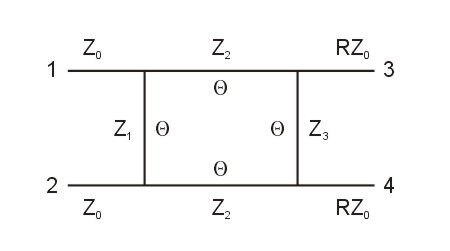
\includegraphics[width=0.5\linewidth]{fig/zad12/coupler_1}
  \caption{Schemat elektryczny sprzęgacza}
  \label{fig:zad12:coupler1}
\end{figure}

\begin{figure}[!htbp]
  \centering
  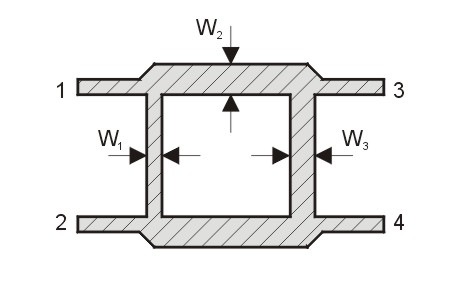
\includegraphics[width=0.5\linewidth]{fig/zad12/coupler_2}
  \caption{Realizacja sprzęgacza z niesymetrycznych linii paskowych}
  \label{fig:zad12:coupler2}
\end{figure}

\section{Rozwiązanie}
\subsection{Projekt sprzęgacza}
Rysunki~\ref{fig:zad12:coupler1} i~\ref{fig:zad12:coupler2} przedstawiają projektowany sprzęgacz.
Sygnał we wrotach 4 jest w przeciwfazie a we wrotach 3 w kwadraturze.
Dwugałęziowy sprzęgacz kierunkowy może transformować impedancję.
Jednak w treści zadania zaznaczono, że jest on obciążony liniami o impedancji charakterystycznej~$Z_0 = 50~\Omega$.
Stąd parametr~$R = 1$.

Współczynnik napięciowego sprzężenia wynosi:
\begin{align}
  k &= \frac{1}{\sqrt{10^{\frac{C}{10}} - 1}} \\
  &= 0.829109611422 \nonumber
\end{align}
Następnie podstawie współczynnika~$k$, wyznacza się wartości impedancji charakterystycznych:
\begin{align}
  Z_1 &= \frac{Z_0}{k} &= 60.3056571908~\Omega \\
  Z_2 &= Z_0\sqrt{\frac{R}{1 + k^2}} &= 38.4908989956~\Omega \\
  Z_3 &= Z_0\frac{R}{k} &= 60.3056571908~\Omega
\end{align}

Wyznaczone impedancje należy zamienić na odcinki niesymetrycznych linii paskowych tak samo jak było to wykonane w rozdziale~\ref{zad6}.
Szerokości ścieżek wynoszą:
\begin{align}
  w1 &= 1.90100127159~mm \nonumber \\
  w2 &= 4.01397627035~mm \nonumber \\
  w3 &= 1.90100127159~mm \nonumber
\end{align}

Podobnie jak w rozdziale~\ref{zad6} aby wyznaczyć długość odcinków ćwierćfalowych, należy obliczyć długość fali rozchodzącej się w linii.
Długość fali zależy od efektywnej przenikalności dielektrycznej~$\epsilon_{eff}$, która jest funkcją wymiarów oraz częstotliwości pracy.
Dlatego obliczono 3 różne długości.
Dla danych z treści zadania mamy:
\begin{align}
  \frac{\lambda_1}{4} &= 3.11142895539~cm \nonumber \\
  \frac{\lambda_2}{4} &= 3.00913769452~cm \nonumber \\
  \frac{\lambda_3}{4} &= 3.11142895539~cm \nonumber 
\end{align}

\subsection{Charakterystyka sprzęgacza}
W celu wyznaczenia charakterystyki częstotliwościowej wartości sprzężenie należy posłużyć się zależnością:
\begin{equation}
  C = 20 \log\Big(\frac{1}{|S_{14}|}\Big) \label{eqn:zad12:C}
\end{equation}

\begin{align}
  S_{14} &= \frac{1}{2} \bigg[ \frac{1}{RD_e + jXD_e} - \frac{1}{RD_o + jXD_o}\bigg] \\
  |S_{14}| &= \frac{1}{2} \bigg[\frac{\sqrt{(RD_o - RD_e)^2 + (XD_o - XD_e)^2}}{(RD_e^2 + XD_e^2)(RD_o^2 + XD_e^2)} \bigg]
\end{align}

Dokładne zależności podane zostały w~\cite{obwody}.
Charakterystykę sprzęgacza zaprezentowano na rys.~\ref{fig:zad12:freq}.

\begin{figure}[!htbp]
  \centering
  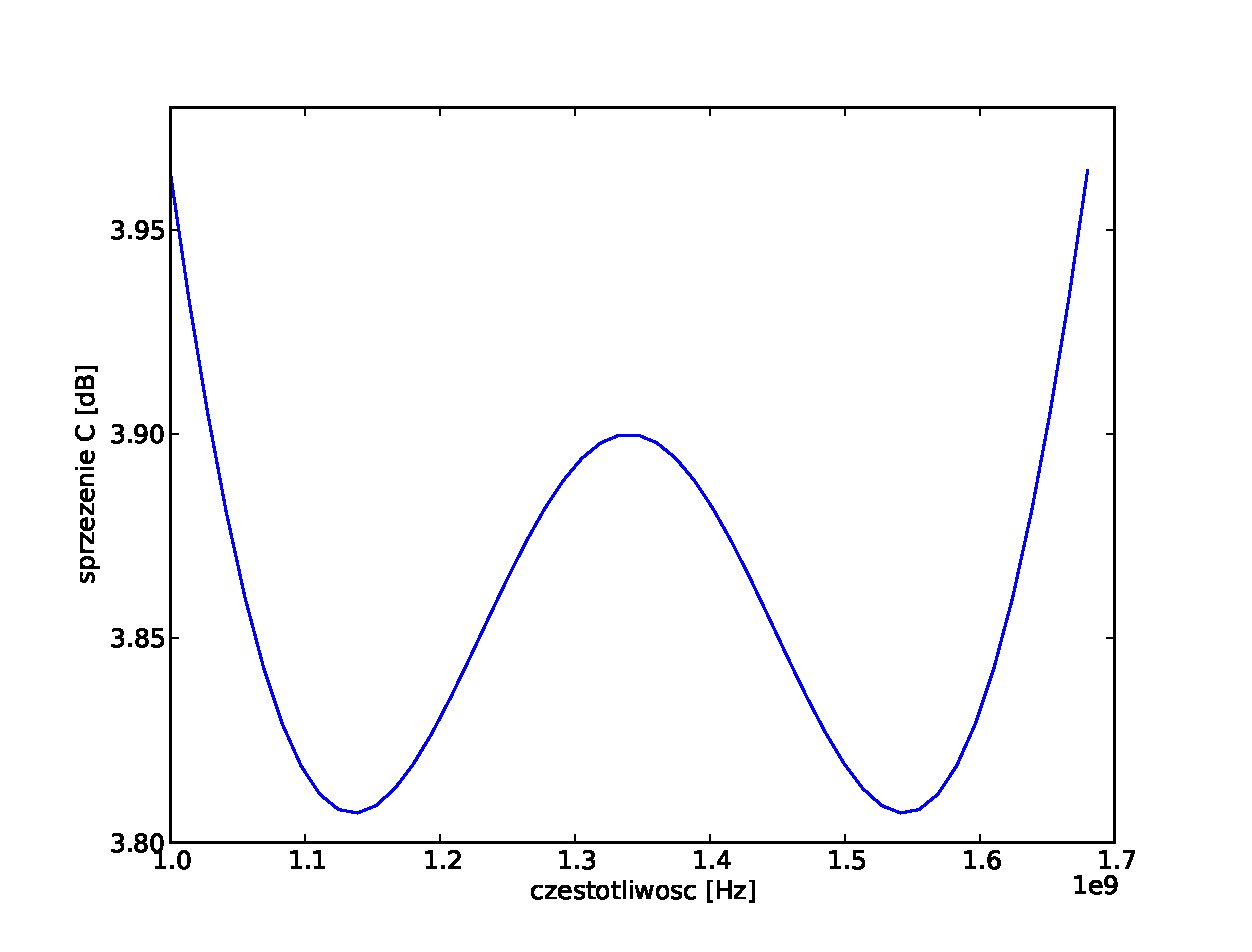
\includegraphics[scale=0.5]{fig/zad12/freq}
  \caption{Charakterystyka częstotliwościowa sprzęgacza}
  \label{fig:zad12:freq}
\end{figure}

\end{document}
